\documentclass{beamer}
\usetheme{InFoMM}
%\setbeamertemplate{blocks}[rounded][shadow=false]
%\addtobeamertemplate{block begin}{\pgfsetfillopacity{0.8}}{\pgfsetfillopacity{1}}
%\setbeamercolor{block title}{bg=blue}
%\setbeamercolor{block title example}{use={normal text,example text},fg=example text.fg!75!normal text.fg,bg=normal text.bg!75!black}

\title{Poor players or dodgy design: How important is the choice of football in the modern game?}
\author{Neil Chada, Peter De Ford, Caoimhe Rooney, Bogdan Toader, \\Florian Wechsung and Tim Whitbread}
\date{Mentor: Dr Timothy Reis}

\usepackage{mathtools}
\usepackage{amsmath}
\mathtoolsset{showonlyrefs}
\usepackage{subfig}
\usepackage[english]{babel}
\usepackage[latin1]{inputenc}

\newcommand{\dr}[1]{\ensuremath{\operatorname{d}\!{#1}}}

\begin{document}
\maketitle

\begin{frame}
  \vspace{1cm}
  During the Football World Cup in 2010 the new ball introduced by Adidas displayed a weird behaviour. Players were confused about the trajectory of the ball, which leads to the following questions:

  \begin{itemize}
    \item Why does it swerve?

    \item Can we model the flight of a football?

    \item Does the choice of ball matter?

    \item Does the location of the game matter?
  \end{itemize}

  \begin{figure}
    \begin{center}
      \includegraphics[scale=0.25]{ball.jpg}
    \end{center}
  \end{figure}
\end{frame}


\begin{frame}
\frametitle{Why does a ball swerve?}
Bernoulli's Theorem for an inviscid flow:
\begin{equation*}
 \frac{\left|\mathbf{v}\right|^2}{2} + p = const.
\end{equation*}
\begin{figure}
          \begin{center}
            \includegraphics[scale=1.6]{bernoulli.png}
          \end{center}
\end{figure}
%(Taken from https://www.comsol.com/blogs/magnus-effect-world-cup-match-ball/)
\end{frame}


\begin{frame}
 \frametitle{Why does a ball swerve?}
The boundary layer on the side of the ball with a greater velocity becomes turbulent and separates from the ball later than the laminar boundary layer. The wake then becomes deflected and so the ball is `pushed' towards the direction of spin.
\begin{figure}
          \begin{center}
            \includegraphics[scale=1]{deflection.png}
          \end{center}
        \end{figure}
\end{frame}

\begin{frame}
\frametitle{Equations}
\begin{itemize}
\item Magnus Force:
  \begin{equation*}
   F_L = \frac83\pi r^2  \rho C_L \vert v \vert^2 ,
  \end{equation*}
where $\rho$ is air density, $v$ is velocity, $r$ is the radius of the ball and $C_L$ is the dimensionless lift coefficient.
\item Drag force:
  \begin{equation*}
   F_D = \frac{1}{2}\pi r^2  \rho C_D \vert v \vert^2,
  \end{equation*}
where $C_D$ is the dimensionless drag coefficient.
\item It is important to note that the Magnus force acts perpendicular to the drag force, which opposes the direction of travel.
\end{itemize}
\end{frame}

\begin{frame}{~}
\begin{itemize}
  \item Considering motion in two-dimensions, we can analyse the path of the ball by looking from above and from the side.
  \item Looking from the side, we consider the following model:
   \begin{align}
    \ddot{x} &= \hphantom{-g}- \frac{1}{m}\frac{\dot{x}}{\left|\mathbf{\dot{x}}\right|}F_D - \frac{1}{m}\frac{\dot{z}}{\left|\mathbf{\dot{x}}\right|}F_L\\
   \ddot{z} &= -g - \frac{1}{m}\frac{\dot{z}}{\left|\mathbf{\dot{x}}\right|}F_D + \frac{1}{m}\frac{\dot{x}}{\left|\mathbf{\dot{x}}\right|}F_L
  \end{align}
\item The lift force $F_L$ is a consequence of top or bottom spin applied to the ball on impact.
\item We can analyse the effects of gravity, drag and spin on the path of the ball.
\end{itemize}
\end{frame}

\begin{frame}{Drag and spin effects on vertical movement}
\begin{figure}
  \begin{center}
     \includegraphics[scale=0.5]{chipped_pass.eps}
  \end{center}
\end{figure}
\end{frame}

\begin{frame}{Varying effects of spinning}
  \begin{figure}
    \begin{center}
      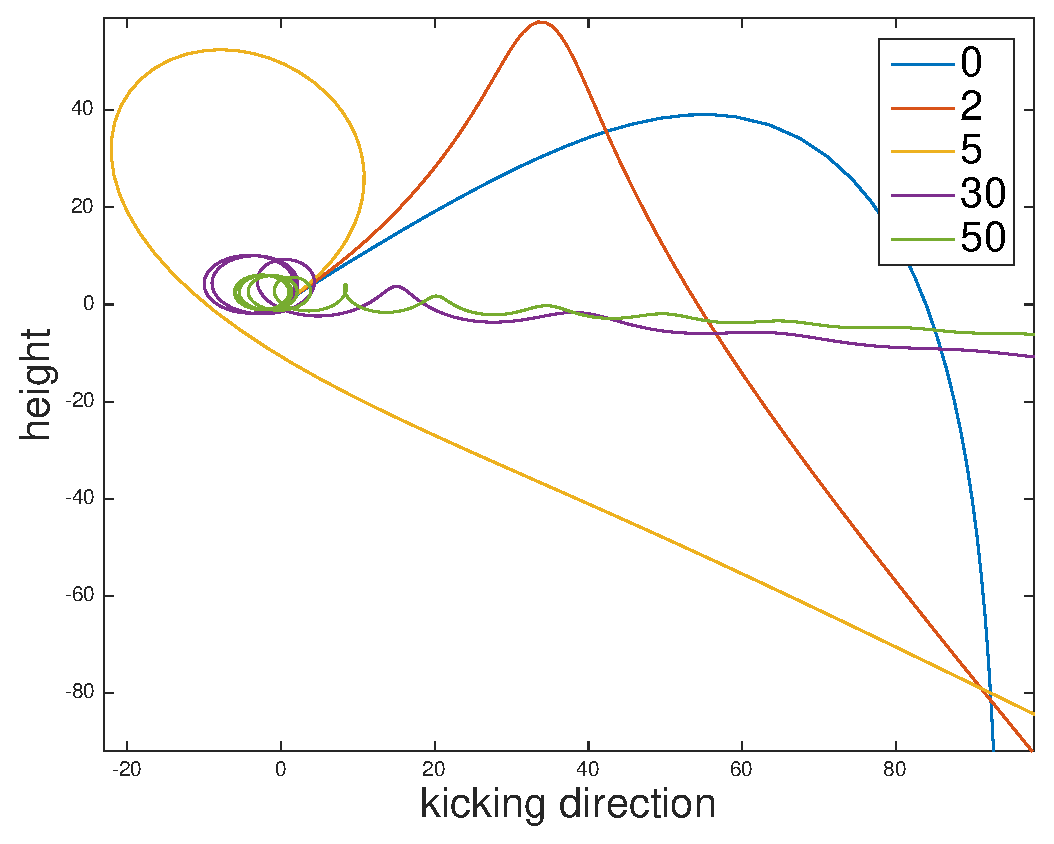
\includegraphics[scale=0.5]{changeRev.eps}
    \end{center}
  \end{figure}
\end{frame}

\begin{frame}{Birds eye view}
\begin{itemize}
\item Looking from above, the Magnus force corresponds to a \textit{lateral force}, which is a consequence of side-spin.
  \begin{center}
    \includegraphics[width=5cm]{rob-carlos-sketch.jpg}
  \end{center}
\item We hence obtain the following model:
\end{itemize}
\begin{align}
    \ddot{x} &= - \frac{1}{m}\frac{\dot{x}}{\left|\mathbf{\dot{x}}\right|}F_D - \frac{1}{m}\frac{\dot{y}}{\left|\mathbf{\dot{x}}\right|}F_L\\
   \ddot{y} &= - \frac{1}{m}\frac{\dot{y}}{\left|\mathbf{\dot{x}}\right|}F_D + \frac{1}{m}\frac{\dot{x}}{\left|\mathbf{\dot{x}}\right|}F_L
  \end{align}
\end{frame}

\begin{frame}{Asymptotics when looking from above}
  \begin{itemize}
    \item Write $K_D v^2 = \frac{F_D}{m}$ and $K_L v^2 = \frac{F_L}{m}$ to obtain
      \begin{gather}
        \ddot x = - K_D \dot x \sqrt{\dot{x}^2 + \dot{y}^2} - K_L \dot y \sqrt{\dot{x}^2 + \dot{y}^2}\\
        \ddot y = - K_D \dot y \sqrt{\dot{x}^2 + \dot{y}^2}  + K_L \dot x \sqrt{\dot{x}^2 + \dot{y}^2}\\
        x(0)=0=y(0) \quad x'(0)=0 \quad y'(0)=v
      \end{gather}
  \end{itemize}
\end{frame}
\begin{frame}{Non-Dimensionalization}
  \begin{itemize}
    \item We rescale: 
  \end{itemize}
  \begin{equation}
    t = \tau \hat t \qquad x= L_1 \hat x \qquad y = L_2 \hat y
  \end{equation}
  and assume that for $y$ only the drag is of relevance.  (Distance towards goal much bigger than sideways motion.)
  Then we obtain 
  \begin{equation}
    \begin{aligned}
      \ddot{\hat x} &= - \dot{\hat y} \sqrt{1 + \frac{L_1^2}{L_2^2}\frac{\dot{\hat x}^2}{\dot{\hat y}^2}} \left( L_2 K_D \dot{\hat x} + \frac{L_2^2 K_L}{L_1} \dot{\hat y} \right)\\
       \ddot{\hat y} &= - \dot{\hat y}^2 L_2 K_D
    \end{aligned}
  \end{equation}
  The equation for $\hat y$ can be solved analytically and can be redimensionalized:
  \begin{equation}
    y(t) = \frac{1}{K_D}\log(1+tvK_D)
  \end{equation}
\end{frame}
\begin{frame}{~}
  Now considering the equation for $\hat x$, we use the following scalings:
  \begin{equation}
    L_1 = K_L L_2^2 \qquad \epsilon = K_D L_2
  \end{equation}
  and write $a= \frac{K_L}{K_D}$.
  That gives 
  \begin{equation}
    \begin{aligned}
    \ddot{\hat x} &= - \dot{\hat y} \sqrt{1+ a^2 \epsilon^2 \frac{\dot{\hat x}^2}{\dot{\hat y}^2}} \left( \epsilon \dot{\hat x} + \dot{\hat y} \right) \\
      &\approx \dot{\hat y} \left(1+ \frac12a^2 \epsilon^2 \frac{\dot{\hat x}^2}{\dot{\hat y}^2}\right) \left( \epsilon \dot{\hat x} + \dot{\hat y} \right)
    \end{aligned}
  \end{equation}
  Now write $\hat x = \hat x^0 + \epsilon \hat x^1  + \ldots$
  and obtain
  \begin{equation}
    \begin{aligned}
      \ddot{{\hat{x}}}^0 &= - \left( \dot{\hat y} \right) ^2\\
      \ddot{\hat x}^1  &= - \dot{\hat y} \dot{\hat x}^0
    \end{aligned}
  \end{equation}
  (both with homogenous boundary condition at zero).
\end{frame}
\begin{frame}{Solving the asymptotics}
    \begin{itemize}
      \item These can be solved and we obtain our solutions:
    \end{itemize}
    \begin{equation}
      \begin{aligned}
        \hat x^0 &=\frac{K_L \log \left(t v K_D+1\right)}{K_D^2}-\frac{t v K_L}{K_D}\\
        \epsilon \hat x^1 &= \frac{v K_L \left(t \log \left(t v K_D+1\right)+\frac{2 \log \left(t v K_D+1\right)}{v K_D}-t\right)}{K_D}-\frac{t v K_L}{K_D}
      \end{aligned}
    \end{equation}
\end{frame}
\begin{frame}{Quality of the Asymptotics}
  \begin{itemize}
    \item Lets consider a kick at $30$m/s with $3$ revolutions per second.
    \item We compare the analytical solution to a numerical solution.
  \end{itemize}
  \begin{center}
    \begin{figure}
      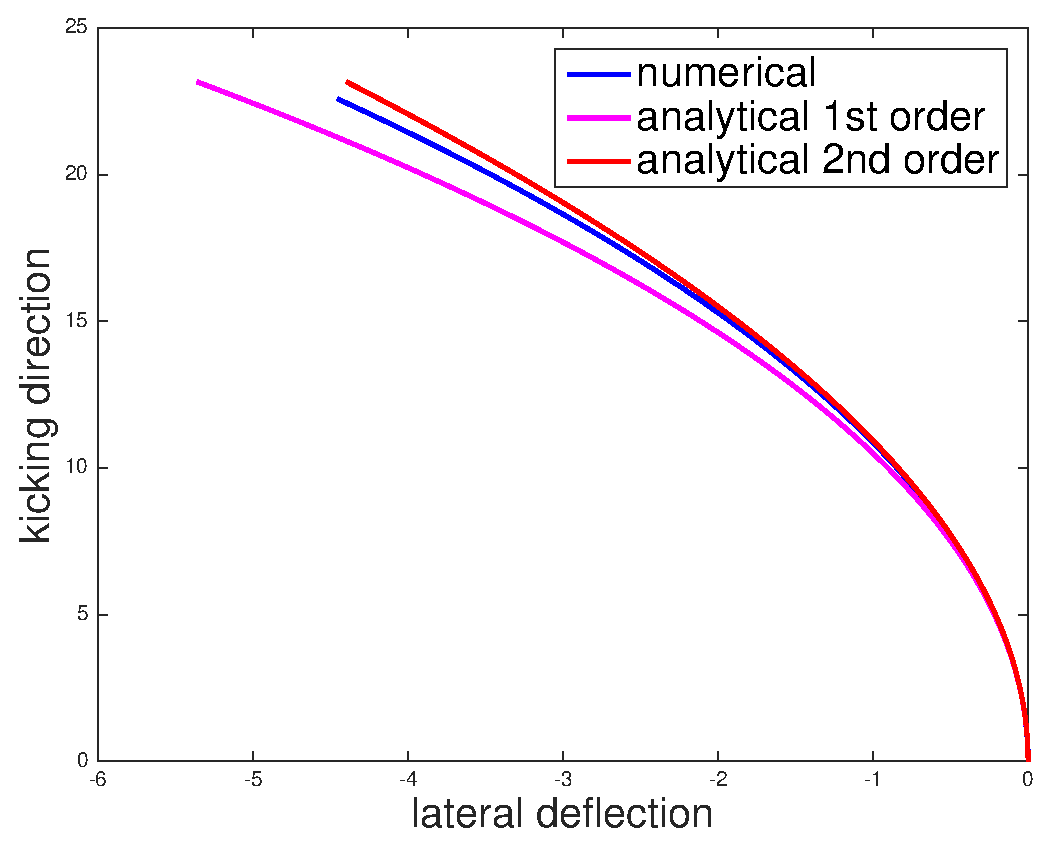
\includegraphics[width=6cm]{numericalVsAnalytical.eps}
      \caption{Numerical vs First-Order vs Second-Order approximation}
    \end{figure}
  \end{center}
\end{frame}
\begin{frame}{Location Changes}
  \begin{itemize}
    \item Changes in air density can change the swerve of a typical free kick by up to a meter!
  \end{itemize}
  \begin{center}
    \begin{figure}
      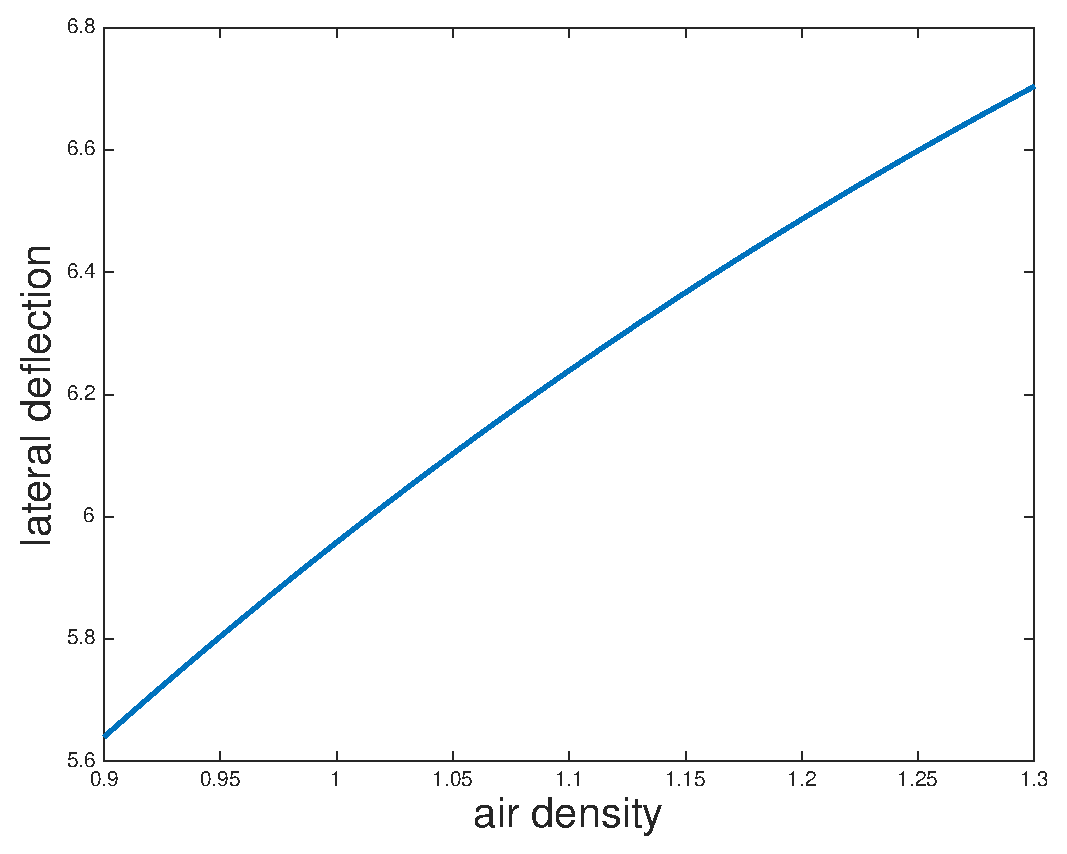
\includegraphics[width=5cm]{densityVar.eps}
      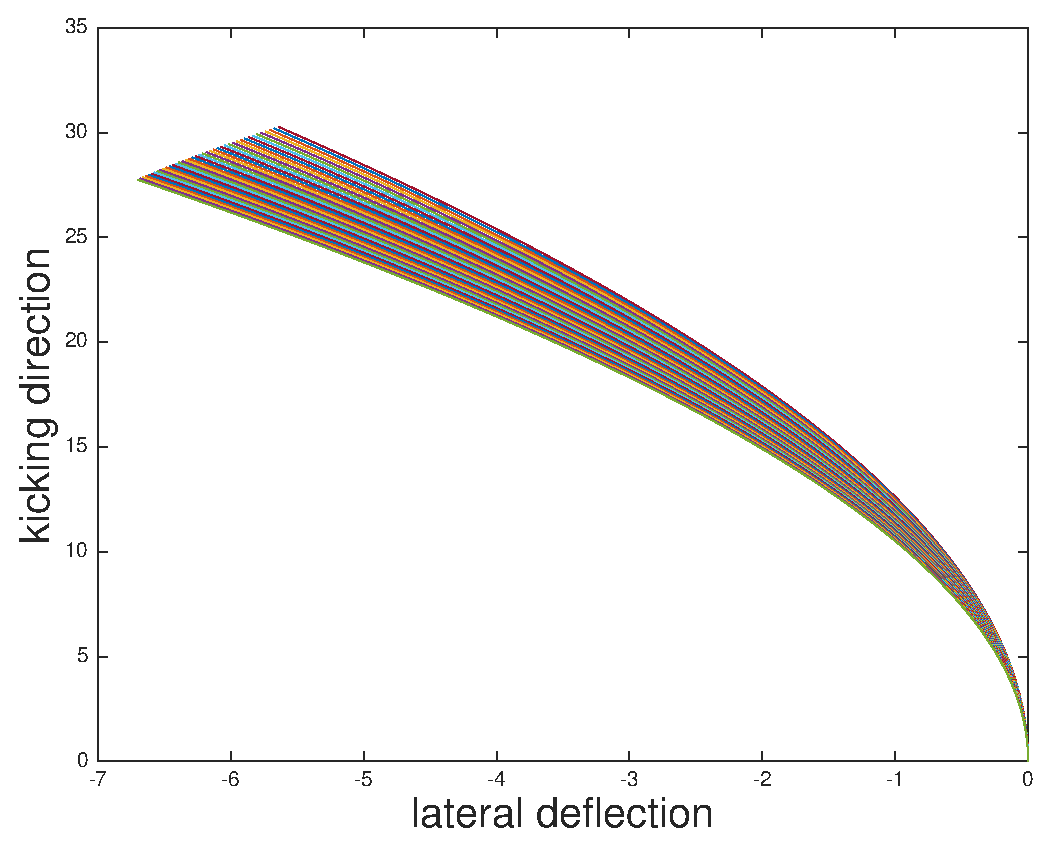
\includegraphics[width=5cm]{densityTraj.eps}
    \end{figure}
  \end{center}
\end{frame}
\begin{frame}{Back to Roberto Carlos...}
  \begin{itemize}
    \item From video analysis we can infer that Robert Carlos freekick had a speed of approximately $30$m/s and $10$ revolutions per second.
    \item Our model gives a deviation from a straig shot of approximately $4$m.
    \item This is coherent with measurements that sports journals have taken.
  \end{itemize}
  \begin{figure}
    \begin{center}
      \includegraphics[width=6.5cm]{rob_cartoon.png}
    \end{center}
  \end{figure}
\end{frame}


\begin{frame}
 \frametitle{Drag crisis}
\begin{itemize}
\item Low Reynolds number (i.e. low velocities): Laminar boundary layer separates from the ball earlier $\rightarrow$ forms wide, low-pressure wake $\rightarrow$ slows down ball.\\\vspace{\baselineskip}
\item Higher Reynolds number (higher velocities): Boundary layer becomes turbulent $\rightarrow$ separates later than in laminar case $\rightarrow$ forms a narrower wake and a lower drag coefficient.\\\vspace{\baselineskip}
\item A fast-moving ball may not slow down as quickly as a goalkeeper might expect.
\end{itemize}
\end{frame}

\begin{frame}
 \frametitle{Other reasons for irratic behaviour}
\begin{itemize}
\item Reverse Magnus effect:
\begin{itemize}
\item The flight of a ball with a low angular velocity (relative to  becomes primarily dependent on the air pressure which is constantly changing. The points where the flow transitions from laminar to turbulent are different on either side of the ball, so the Magnus effect can reverse, leading to a `knuckle ball' effect.\\\vspace{\baselineskip}
\item The smoothness of the ball changes the position of these transition points: A ball with a rougher surface or stitching is more likely to follow the `standard' positive Magnus effect.
\end{itemize}
\end{itemize}
\end{frame}

\begin{frame}{Conclusions --- What have we done?}
  \begin{itemize}
    \item 2D Models for side view and birds eye view.
    \item Asymptotic solution for the birds eye model case when the deviation from a straight shot is small.
    \item Numerical solution for both models including the drag crisis. 
    \item 3D Model including drag crisis.
    \item Numerical solution for 3D model. 
  \end{itemize}
\end{frame}
\begin{frame}{Objectives}
  \begin{itemize}
    \item Why does the ball swerve?
      \begin{itemize}
        \item Magnus effect.
      \end{itemize}
      \item Can we model the flight of a football?
      \begin{itemize}
        \item Yes. In 2D (numerical \& analytical) and 3D (numerical).
      \end{itemize}
      \item Does the location matter?
      \begin{itemize}
        \item Yes. The density of the air can change the amount of swerve drastically.
      \end{itemize}
      \item Does the choice of ball matter?
      \begin{itemize}
        \item Yes. Smoother balls have the drag crisis at higher velocities.
      \end{itemize}
      \item Can we explain oscillations in the flight?
      \begin{itemize}
        \item Only speculate...
      \end{itemize}
  \end{itemize}
\end{frame}
\begin{frame}{Next steps}
  \begin{itemize}
    \item Higher order asymtotics.
    \item 3D analytical solution.
    \item Better drag crisis model.
    \item Full CFD.
    \item Model any other famous freekicks?
  \end{itemize}
\end{frame}
\end{document}






